%=====================================================
\section{Set Operations}
%=====================================================


%-----------------------------------------------------
\begin{frame}{Set Operations}

\begin{block}{Definition}

\vspace{0.1cm}

Set operations combine or modify sets to create new sets.
\[
A,B \rightarrow \text{New Set}
\]

\end{block}

\vspace{0.1cm}

Common set operations:

\begin{enumerate}
    \item Union
    \item Intersection
    \item Set Difference
    \item Symmetric Difference
    \item Complement
    \item Cartesian Product
\end{enumerate}


\end{frame}


%-----------------------------------------------------
\begin{frame}{Union of Sets}

\begin{block}{Mathematical Definition}

\vspace{0.1cm}

The union of two sets contains all the elements that belong
to either set.

\[
A\cup B=\{x\mid x\in A\lor x\in B\}
\]

\end{block}

\vspace{0.1cm}

Example:
\[
A=\{1,2,3\}
\]
\[
B=\{3,4,5\}
\]
\[
A\cup B=\{1,2,3,4,5\}
\]

Example:
Combining two feature sets from different datasets.
\[
Features =
A\cup B
\]

\end{frame}

%-----------------------------------------------------
\begin{frame}{Intersection of Sets}

\begin{block}{Mathematical Definition}

\vspace{0.1cm}

The intersection contains elements common to both sets.

\[
A\cap B=\{x\mid x\in A\land x\in B\}
\]

\end{block}

Example:
\[
A=\{Python,Java,C++\}
\]
\[
B=\{Python,R,Java\}
\]
\[
A\cap B=\{Python,Java\}
\]

Example:
Common features selected by two machine learning models.
\[
Selected=A\cap B
\]

\end{frame}



%-----------------------------------------------------
\begin{frame}{Set Difference}

\begin{block}{Mathematical Definition}

\vspace{0.1cm}

The difference of two sets contains elements present in
one set, but not in the other.

\[
A-B=\{x\mid x\in A\land x\notin B\}
\]

\end{block}

Example:
\[
A=\{1,2,3,4,5\}
\]
\[
B=\{3,4,5,6,7\}
\]
\[
A-B=\{1,2\}
\]

Example:
Removing already processed data samples:
\[
NewData=Dataset-Processed
\]

\end{frame}

%-----------------------------------------------------
\begin{frame}{Symmetric Difference}

\begin{block}{Mathematical Definition}

\vspace{0.1cm}

The symmetric difference contains elements that belong
to exactly one of the sets.

\[
A\triangle B=(A-B)\cup(B-A)
\]

\end{block}

Example:
\[
A=\{1,2,3\}
\]
\[
B=\{3,4,5\}
\]
\[
A\triangle B=\{1,2,4,5\}
\]

Example:
Files modified in either branch but not both.
\[
Changes=A\triangle B
\]

\end{frame}

%-----------------------------------------------------
\begin{frame}{Complement of a Set}

\begin{block}{Mathematical Definition}

\vspace{0.1cm}

The complement contains elements from the universal set
that are not present in the given set.
\[
A^c=U-A
\]

\end{block}

Example:
\[
U=\{1,2,3,4,5\}
\]
\[
A=\{1,2\}
\]
\[
A^c=\{3,4,5\}
\]

Example:
Classification errors:
\[
Correct^c = Incorrect
\]

\end{frame}

%-----------------------------------------------------
\begin{frame}{Cartesian Product}

\begin{block}{Mathematical Definition}

\vspace{0.1cm}

Cartesian product creates ordered pairs.
\[
A\times B=
\{(a,b)\mid a\in A,\ b\in B\}
\]

\end{block}
Example:
\[
A=\{1,2\}
\]
\[
B=\{Python,Java\}
\]
\[
A\times B=
\{
(1,Python),
(1,Java),
(2,Python),
(2,Java)
\}
\]

Example:
Input-output pairs in supervised learning:
\[
(X,Y)\;where
\]
\[
X\times Y\;represents \;possible\; input-label\; combinations.
\]

\end{frame}

%-----------------------------------------------------
\begin{frame}{Set Operations using Venn Diagrams}

\begin{center}
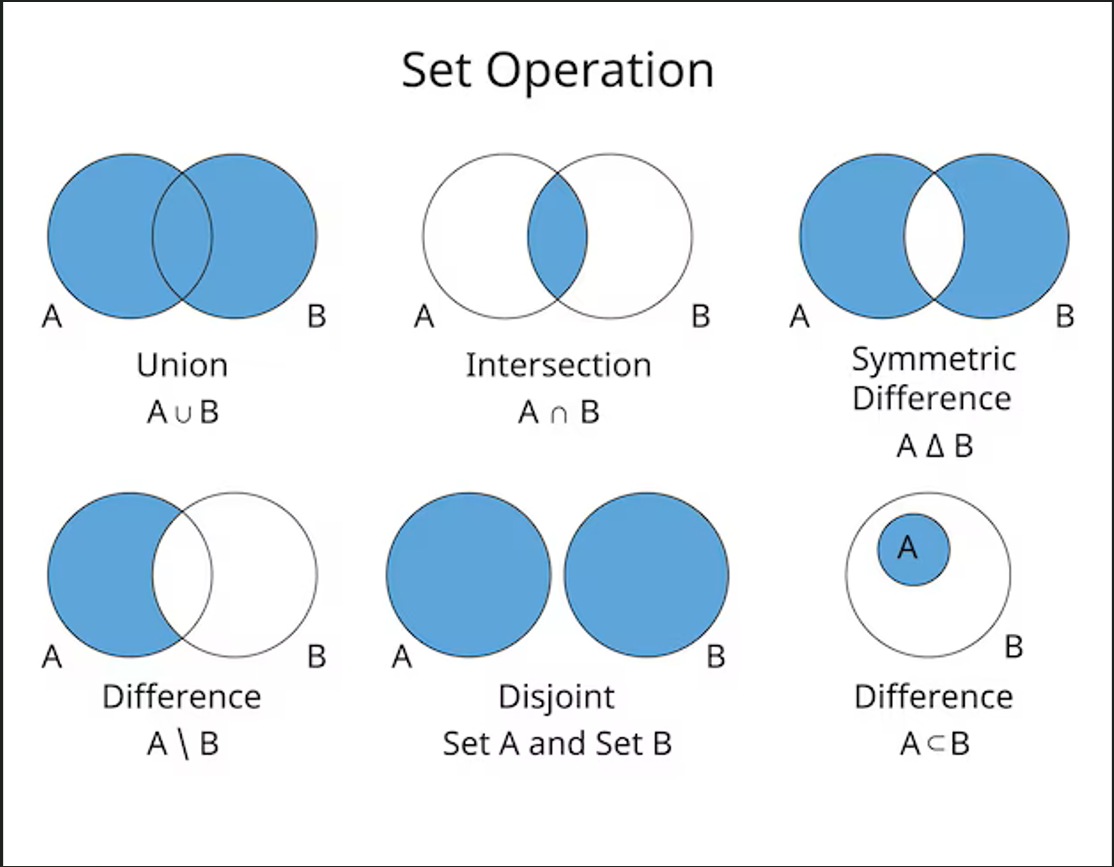
\includegraphics[width=0.7\linewidth]{images/operations.png}
\end{center}

\end{frame}